\documentclass[11pt]{article}
\usepackage[margin=1in]{geometry}
\usepackage{amsmath,amssymb,amsthm,bm}
\usepackage{graphicx}
\usepackage{booktabs}
\usepackage{xcolor}
\usepackage[colorlinks=true,linkcolor=blue,citecolor=blue,urlcolor=blue]{hyperref}
\usepackage{caption}
\captionsetup{font=small,labelfont=bf}

\newtheorem{definition}{Definition}
\newtheorem{proposition}{Proposition}

\newcommand{\A}{\mathcal{A}}
\newcommand{\x}{\bm{x}}
\newcommand{\z}{\bm{z}}

\title{\bf The shapes a machine draws: a recalibration-invariant relational
description of multi-physics operation}
\author{Sehaj Singh}
\date{\today}

\begin{document}
\maketitle

\begin{abstract}
\noindent
A machine under load moves along a coupled thermal, mechanical and electrical
trajectory, and every pair of its channels traces a shape as it goes. Those
shapes are not decoration, they carry the physics: a tight single valued curve
means an instantaneous constraint, an oriented loop means a lag with a
direction, a branched cloud means a hidden third variable, a stepped scatter
means a switching command. We make that observation into a measurable object.
Each channel pair gets nine \emph{atoms}, scalar descriptors of association,
functional strength, nonlinearity, asymmetry, oriented hysteresis, jump share,
timescale ratio, support occupancy and scaling exponent, and the whole array
over all pairs is the operating atlas of one unit. Eight of the nine are
computed on within-unit ranks and are therefore exactly invariant to any
strictly increasing recalibration of each channel separately, which we verify
to machine precision end to end on real telemetry rather than in principle.
On a real permanent magnet motor bench, one machine recorded in 40 separate
measurement sessions, the atlas identifies which session a held out record came
from at 32.5\% top-1 against 2.5\% chance, where the same construction reduced
to its first atom, a Spearman correlation matrix, reaches 7.5\%. We are careful
about the scope of that: it distinguishes operating episodes of one machine, and
on simulated fleets of genuinely distinct machines the same test gives a much
weaker 6 to 15\% against 1.2\% chance, statistically indistinguishable from a
per-channel baseline. The atom carrying most of that identity is
the oriented hysteresis, the signed L\'evy area, which is exactly the quantity
a correlation matrix cannot represent because correlation is symmetric and the
L\'evy area is antisymmetric. Collapsing each unit's atlas to nine quantiles
per atom gives a class signature of fixed length whatever the channel count,
and that signature assigns six classes spanning a motor bench, an air
compressor, two fault states of a pump rig, a turbofan and a basket of traded
assets at $93.6\pm1.4\%$ against a $28.6\%$ majority, with every error falling
between the two fault states of the same rig.

We are equally specific about what the construction does not buy. Against a
strong non-relational baseline, per channel means, standard deviations, skews
and kurtoses, the in-distribution gain is modest, 32.5\% against 25.0\%. The
separation appears only when instrumentation changes, where the atlas is
unmoved at 32.5\% and the baseline falls to 5.0\%. Atoms also need roughly
$10^3$ to $10^4$ samples per unit before they stop being noise, which is why
the same method returns almost nothing on C-MAPSS, whose units are 200 cycles
long. And the invariance that makes the atlas survive re-instrumentation is
what makes it blind to absolute level, so a machine that simply runs hotter is
invisible to it. Invariance and identifiability trade off, and we quantify the
trade rather than resolve it.
\end{abstract}

\section{Introduction}

A servo joint accelerating a payload dissipates ohmic heat into a winding whose
rising temperature derates the torque available to the next command, on a
thermal time constant three decades slower than the control loop that issued
it. Watch any one channel and you see a line wandering. Watch two of them
against each other and you see a shape, and the shape is where the coupling
lives, because a lag between torque and winding temperature is not visible in
either trace on its own but shows up immediately as an oriented loop in the
plane they span.

Practitioners already know this, which is why torque-speed envelopes and
pressure-volume diagrams and Nyquist plots exist. What has not been done is to
treat the whole set of such shapes, across every pair of channels and across
operating conditions, as a single object attached to a specific machine, and to
ask what that object is good for. That is what we do here. We call the array of
shape descriptors for one machine its \emph{index of operations}, and the
class-level structure shared across machines of the same kind its \emph{index
of operators}.

The proposal is easy to state and easy to get wrong, so it is worth being
precise about what would count as evidence. If the shapes are a property of the
machine, then an atlas built from one stretch of a machine's life should
identify that same machine from a different stretch, run under a different
workload, against a lineup of its siblings. If the shapes are merely a property
of the duty cycle, the same test will fail while looking superficially healthy
on any in-distribution accuracy metric. We therefore lead with identification
rather than with prediction, because identification is the claim that
discriminates.

Two scope limits are worth stating at the outset rather than discovering
halfway through. First, public industrial telemetry almost never contains many
nominally identical units, so the strongest version of this test, distinguishing
one physical machine from its siblings, can only be run on simulation, and there
the answer is weak. What the real data supports is distinguishing operating
episodes of a machine, distinguishing kinds of machine, and diagnosing faults.
Second, and more usefully, the property that does survive contact with real
hardware is not identification at all but invariance: the description does not
move when the instrumentation is changed, and the standard alternative does.
That is what this paper is finally about.

\subsection{Relation to existing work}

Four literatures touch this and none of them do it.

Path signatures from rough path theory give a canonical description of the
shape of a multivariate path, and their depth-2 term is precisely the L\'evy
area we use as one of nine atoms. Signatures are the closest formal ancestor
of this work. They are also combinatorially expensive in the channel count,
they carry no notion of how single valued or how discontinuous a relation is,
and they are not organised into a class prototype with per unit deformations.

Topological data analysis supplies the support and loop structure of a point
cloud, which is close to our occupancy atom, but discards orientation and
scaling, and orientation is the part that turns out to matter most.

Recurrence quantification analysis and its cross and multidimensional variants
quantify how two systems revisit shared states. They are computed on a single
pair at a time and are not invariant to recalibration.

Graph neural networks for machinery prognostics learn an adjacency over
sensors. The adjacency is a fitted nuisance parameter, not a readable physical
statement, it is specific to the training fleet, and nothing in it survives a
sensor swap.

The closest structural analogue is outside engineering entirely. Functional
connectome fingerprinting identifies individual people from the pattern of
correlations between brain regions, and reports that individual identity is
diffusely spread over many edges. Our construction is that idea for machines,
with the crucial difference that a correlation is only the first of nine
descriptors, and, as we show, by some distance not the most informative one.

\section{The operating atlas}

\subsection{Atoms}

A unit presents $d$ channels sampled over time. For each unordered pair
$(i,j)$ we compute nine scalars. Write $u_k$ for the within-unit rank transform
of channel $k$, mapped to $(0,1)$ with ties averaged.

\begin{enumerate}
\item $\rho$, the Spearman correlation, the signed monotone association. This
is the classical relational feature and serves as our reduced baseline.
\item $\eta$, the correlation ratio, the largest fraction of one channel's
variance explained by binning on the other. It asks whether the relation is a
single valued curve at all, which a correlation coefficient cannot see.
\item $\mathrm{nlgap} = \eta - \rho^2$, the part of the dependence that is not
monotone.
\item $\mathrm{asym}$, the difference between the two directional correlation
ratios, which says which channel is more nearly a function of the other.
\item $\mathrm{levy}$, the signed L\'evy area normalised by the total absolute
area swept,
\[
\mathrm{levy}_{ij}
= \frac{\sum_t \left(u_i\,\mathrm{d}u_j - u_j\,\mathrm{d}u_i\right)}
       {\sum_t \left|u_i\,\mathrm{d}u_j - u_j\,\mathrm{d}u_i\right|}\ \in[-1,1].
\]
Its sign is a lead-lag direction and its magnitude is how consistently the pair
circulates. A single valued instantaneous relation encloses zero net area
however far it travels, while a lagged one traces a loop with a definite sense.
Normalising by the signed area per step instead would make the atom decay like
$1/T$ under refinement, which is wrong, because what identifies a machine is
the orientation and not the duration.
\item $\mathrm{jump}$, the share of the pair's total absolute co-movement
carried by tail increments, with each channel thresholded on its own tail.
\item $\tau$, the log ratio of the two channels' autocorrelation times.
\item $\mathrm{fill}$, the fraction of a $16\times16$ quantile grid the joint
cloud occupies.
\item $\beta$, the log-log slope of one channel against the other over quantile
binned medians. This is the one deliberately scale dependent atom, kept because
it reads a physical law straight off the shape, since ohmic heating gives
$\Delta T\sim\tau^2$ and therefore $\beta\approx2$ on a torque-temperature
pair.
\end{enumerate}

\subsection{Exact invariance under recalibration}

\begin{proposition}
Let $\phi_1,\dots,\phi_d$ be strictly increasing injective maps applied
channelwise. The first eight atoms are unchanged.
\end{proposition}

The argument is immediate, since each of the eight is a function of the
channelwise ranks alone and an injective increasing map preserves ranks
exactly. The content is not the proposition but the fact that it survives
contact with real data, which took three corrections that are worth recording
because each looked like a property of the method and was in fact a defect of
the implementation.

Cells, the partition of the record by operating point, were first defined by
each unit's own leading principal direction. A principal direction is
determined only up to sign and is fitted per unit, so ``cell 1'' meant a
different operating condition for every machine and half the fleet had its
cells in reverse order. Cells are now quantiles of a load coordinate built from
the mean of per channel ranks, which is itself invariant, so the cell
assignment inherits the invariance rather than breaking it.

Ties were originally broken by array order. A strictly increasing map cannot
reorder distinct values, but in floating point it can collapse two nearby
values onto the same float, and an order based tiebreak then swaps those
samples relative to the unwarped ranking. Averaging ties removes this.

The recalibration model itself was wrong. Composing a power law with a logistic
squash is monotone on paper, but with the exponent drawn from
$\exp(\mathcal{N}(0,0.8))$ it routinely reached $10$, which sends most of the
unit interval below $10^{-10}$ and onto the flat tail of the logistic,
collapsing thousands of distinct readings onto one float. That destroys
information rather than relabelling it, and no invariant of any kind could have
survived it. The model is now a monotone piecewise linear map through random
increasing knots with segment slopes bounded away from zero, which is what a
replacement sensor with a different response curve actually looks like.

With those three corrected, the measured shift of all eight invariant atoms
under random per channel recalibration is $0.00\times10^{0}$, exactly, on
continuous data, while $\beta$ moves as designed.

\subsection{A parity argument for why correlation cannot substitute}

The claim that a correlation matrix cannot express a lead-lag direction is
usually argued from the symmetry of the pair $(i,j)$. There is a sharper
statement available in terms of time reversal, and it explains the empirical
ranking of the atoms rather than merely asserting it.

\begin{proposition}
Let $\mathcal{R}$ denote reversal of the record, $x(t)\mapsto x(T-t)$. Any
statistic that is a functional of the joint distribution of simultaneous
channel values alone is invariant under $\mathcal{R}$, since reversal permutes
the samples and leaves that distribution fixed. Correlation of any kind,
mutual information, distance correlation, coherence magnitude, copula based
dependence measures and the geometry of the joint support are all of this form.
The normalised signed L\'evy area is not: under $\mathcal{R}$ it changes sign.
\end{proposition}

The atom vocabulary therefore splits into an even sector and an odd sector, and
the split is exact rather than approximate. Measured on the 40 real motor
sessions, eight of the nine atoms reproduce themselves under reversal to
between $10^{-15}$ and $10^{-11}$, while $\mathrm{levy}$ satisfies
$\mathrm{levy}(\mathcal{R}x) = -\mathrm{levy}(x)$ to $4.7\times10^{-14}$ and is
the only atom that does.

This is the reason $\mathrm{levy}$ carries the most identification. A machine's
defining multi-physics behaviour is a lag with a direction, torque heating a
winding that then derates the torque, and lag is precisely the content of the
odd sector. Every descriptor in the standard relational toolkit lives in the
even sector, so the odd sector is exactly the information that toolkit cannot
reach, and it is therefore maximally non-redundant with it. An even statistic
cannot distinguish a lag from a lead however it is scaled or normalised,
because reversing the record leaves it numerically unchanged.

\section{Results}

\begin{figure}[t]
\centering
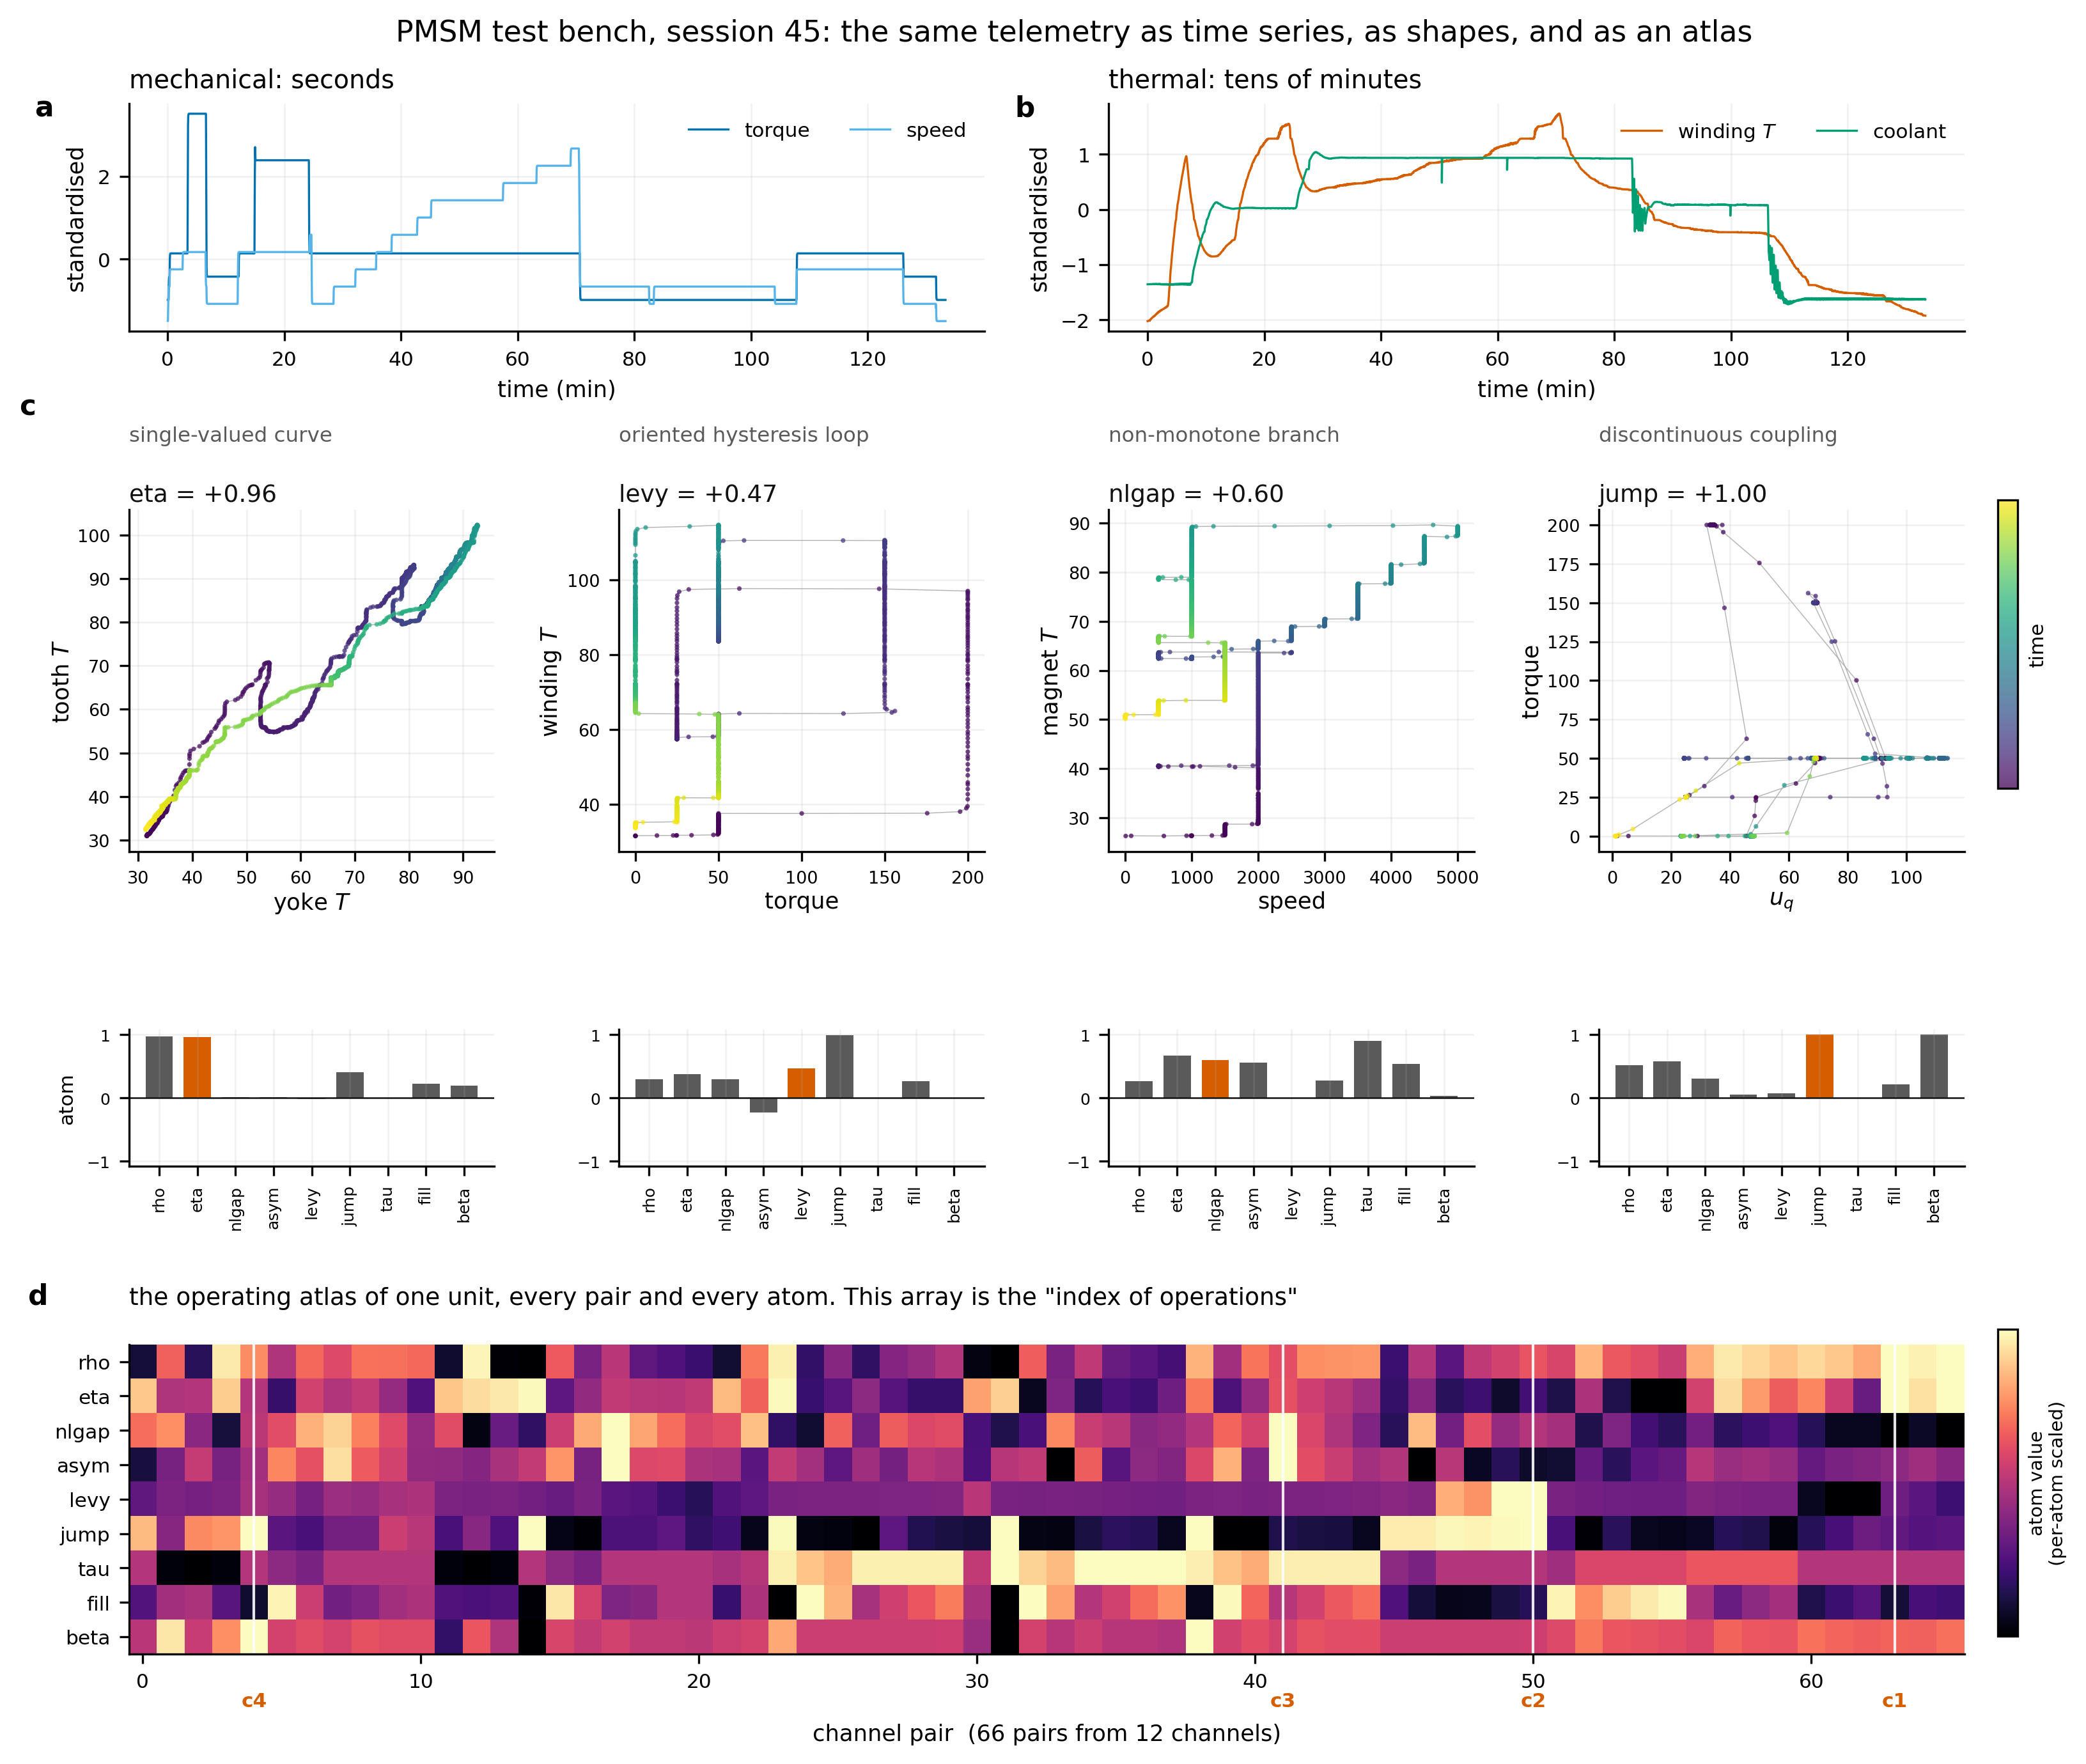
\includegraphics[width=\textwidth]{../atlas/fig1_concept.png}
\caption{The same telemetry three ways. \textbf{a,b} The conventional view,
mechanical channels moving on seconds against thermal channels moving on tens
of minutes. \textbf{c} Four channel pairs and the shapes they trace, each the
arg-max of one atom on this session so the panels show what the method found
rather than what was chosen for it, with the nine atoms of each pair below.
The torque against winding temperature pair encloses an oriented loop at
$\mathrm{levy}=+0.47$, which is the thermal lag made visible. \textbf{d} The
whole atlas, every pair by every atom.}
\end{figure}

\subsection{The atoms report the mechanism}

On a synthetic rig with a known answer, a channel and its causal first order
lag give $\mathrm{levy}=0.23$ while every other pair sits below $0.02$, and a
channel against its own square gives $\rho=0.055$ with
$\mathrm{nlgap}=0.96$, which is a dependence a correlation coefficient reports
as absent. A centred moving average, by contrast, gives $\mathrm{levy}=0$ to
three decimals, correctly, because a zero phase filter encloses no area.

\subsection{Operating episodes are identifiable from their relational geometry}

A point of scope first, because it is easy to get wrong and we got it wrong in
an earlier draft. The permanent magnet motor benchmark is \emph{one} 52\,kW
machine on one test bench, recorded in 69 separate measurement sessions. What
follows therefore shows that distinct operating episodes of a single machine are
identifiable from their relational geometry. It does not show that distinct
physical machines are, and the experiment that speaks to that, the simulated
fleets in Section~\ref{sec:fleet}, gives a much weaker answer. Public
industrial telemetry very rarely contains many nominally identical units, which
is a real limitation on what anyone can claim from it, ourselves included.

\emph{(PMSM bench, 40 sessions of one machine, $1.6\times10^4$ samples each.)}
Atlases are built from the first half of each session and matched against
atlases from the second half, so the target has to be recognised from a
different stretch of its own operating history. Results are in
Table~\ref{tab:fp}.

\begin{table}[t]
\centering
\begin{tabular}{lrrr}
\toprule
feature set & top-1 & percentile rank & top-1 after recalibration \\
\midrule
atlas, invariant 8 atoms  & 32.5\% & 90.0\% & \textbf{32.5\%} \\
full atlas, 9 atoms       & 27.5\% & 89.2\% & --- \\
per channel marginals     & 25.0\% & 82.6\% & \textbf{5.0\%} \\
$\rho$ alone (correlation matrix) & 7.5\% & 71.4\% & --- \\
chance                    & 2.5\%  & 50.0\% & 2.5\% \\
\bottomrule
\end{tabular}
\caption{Identification of 40 measurement sessions of one real motor from held out telemetry, and
the same after an independent strictly increasing warp is applied to every
channel of the held out half.}
\label{tab:fp}
\end{table}

Three things in that table are worth separating, because only one of them is
the headline and it is not the one we expected.

Against the reduced form of our own construction the gain is large. A Spearman
correlation matrix, which is what the relational feature literature actually
uses, reaches 7.5\% where the full atom set reaches 32.5\%, so most of what is
identifying about a machine's relational geometry is not in its correlations.
The single most informative atom is the oriented hysteresis, and that is not an
accident of this dataset, because correlation is a symmetric functional of a
pair while the L\'evy area is antisymmetric, so no correlation based descriptor
can express a lead-lag direction at all. On a machine whose defining physics is
that torque heats a winding which then derates the torque, the direction of
circulation is the physics.

Against a genuinely strong baseline the in-distribution gain is small. Per
channel means, standard deviations, skews and kurtoses reach 25.0\%, within
striking distance of the atlas at 32.5\%, and any claim that relational
geometry is necessary for identification in a stable fleet would be
overstating what we measured.

The separation appears when the instrumentation changes. Under an independent
monotone warp per channel the atlas is unmoved at 32.5\%, exactly, while the
marginal baseline falls from 25.0\% to 5.0\%, a factor of five, because
everything it encodes is a magnitude and every magnitude has been relabelled.
That is the regime the construction is for, and it is worth being precise that
it is the only regime in which we can show it clearly winning.

Finally, the invariant eight atoms beat all nine at 32.5\% against 27.5\%.
Including $\beta$, the one scale dependent atom, actively hurts, which is
consistent with it being the weakest atom individually and is a reason to keep
it out of the identification pipeline and reserve it for physical readout.

\begin{figure}[t]
\centering
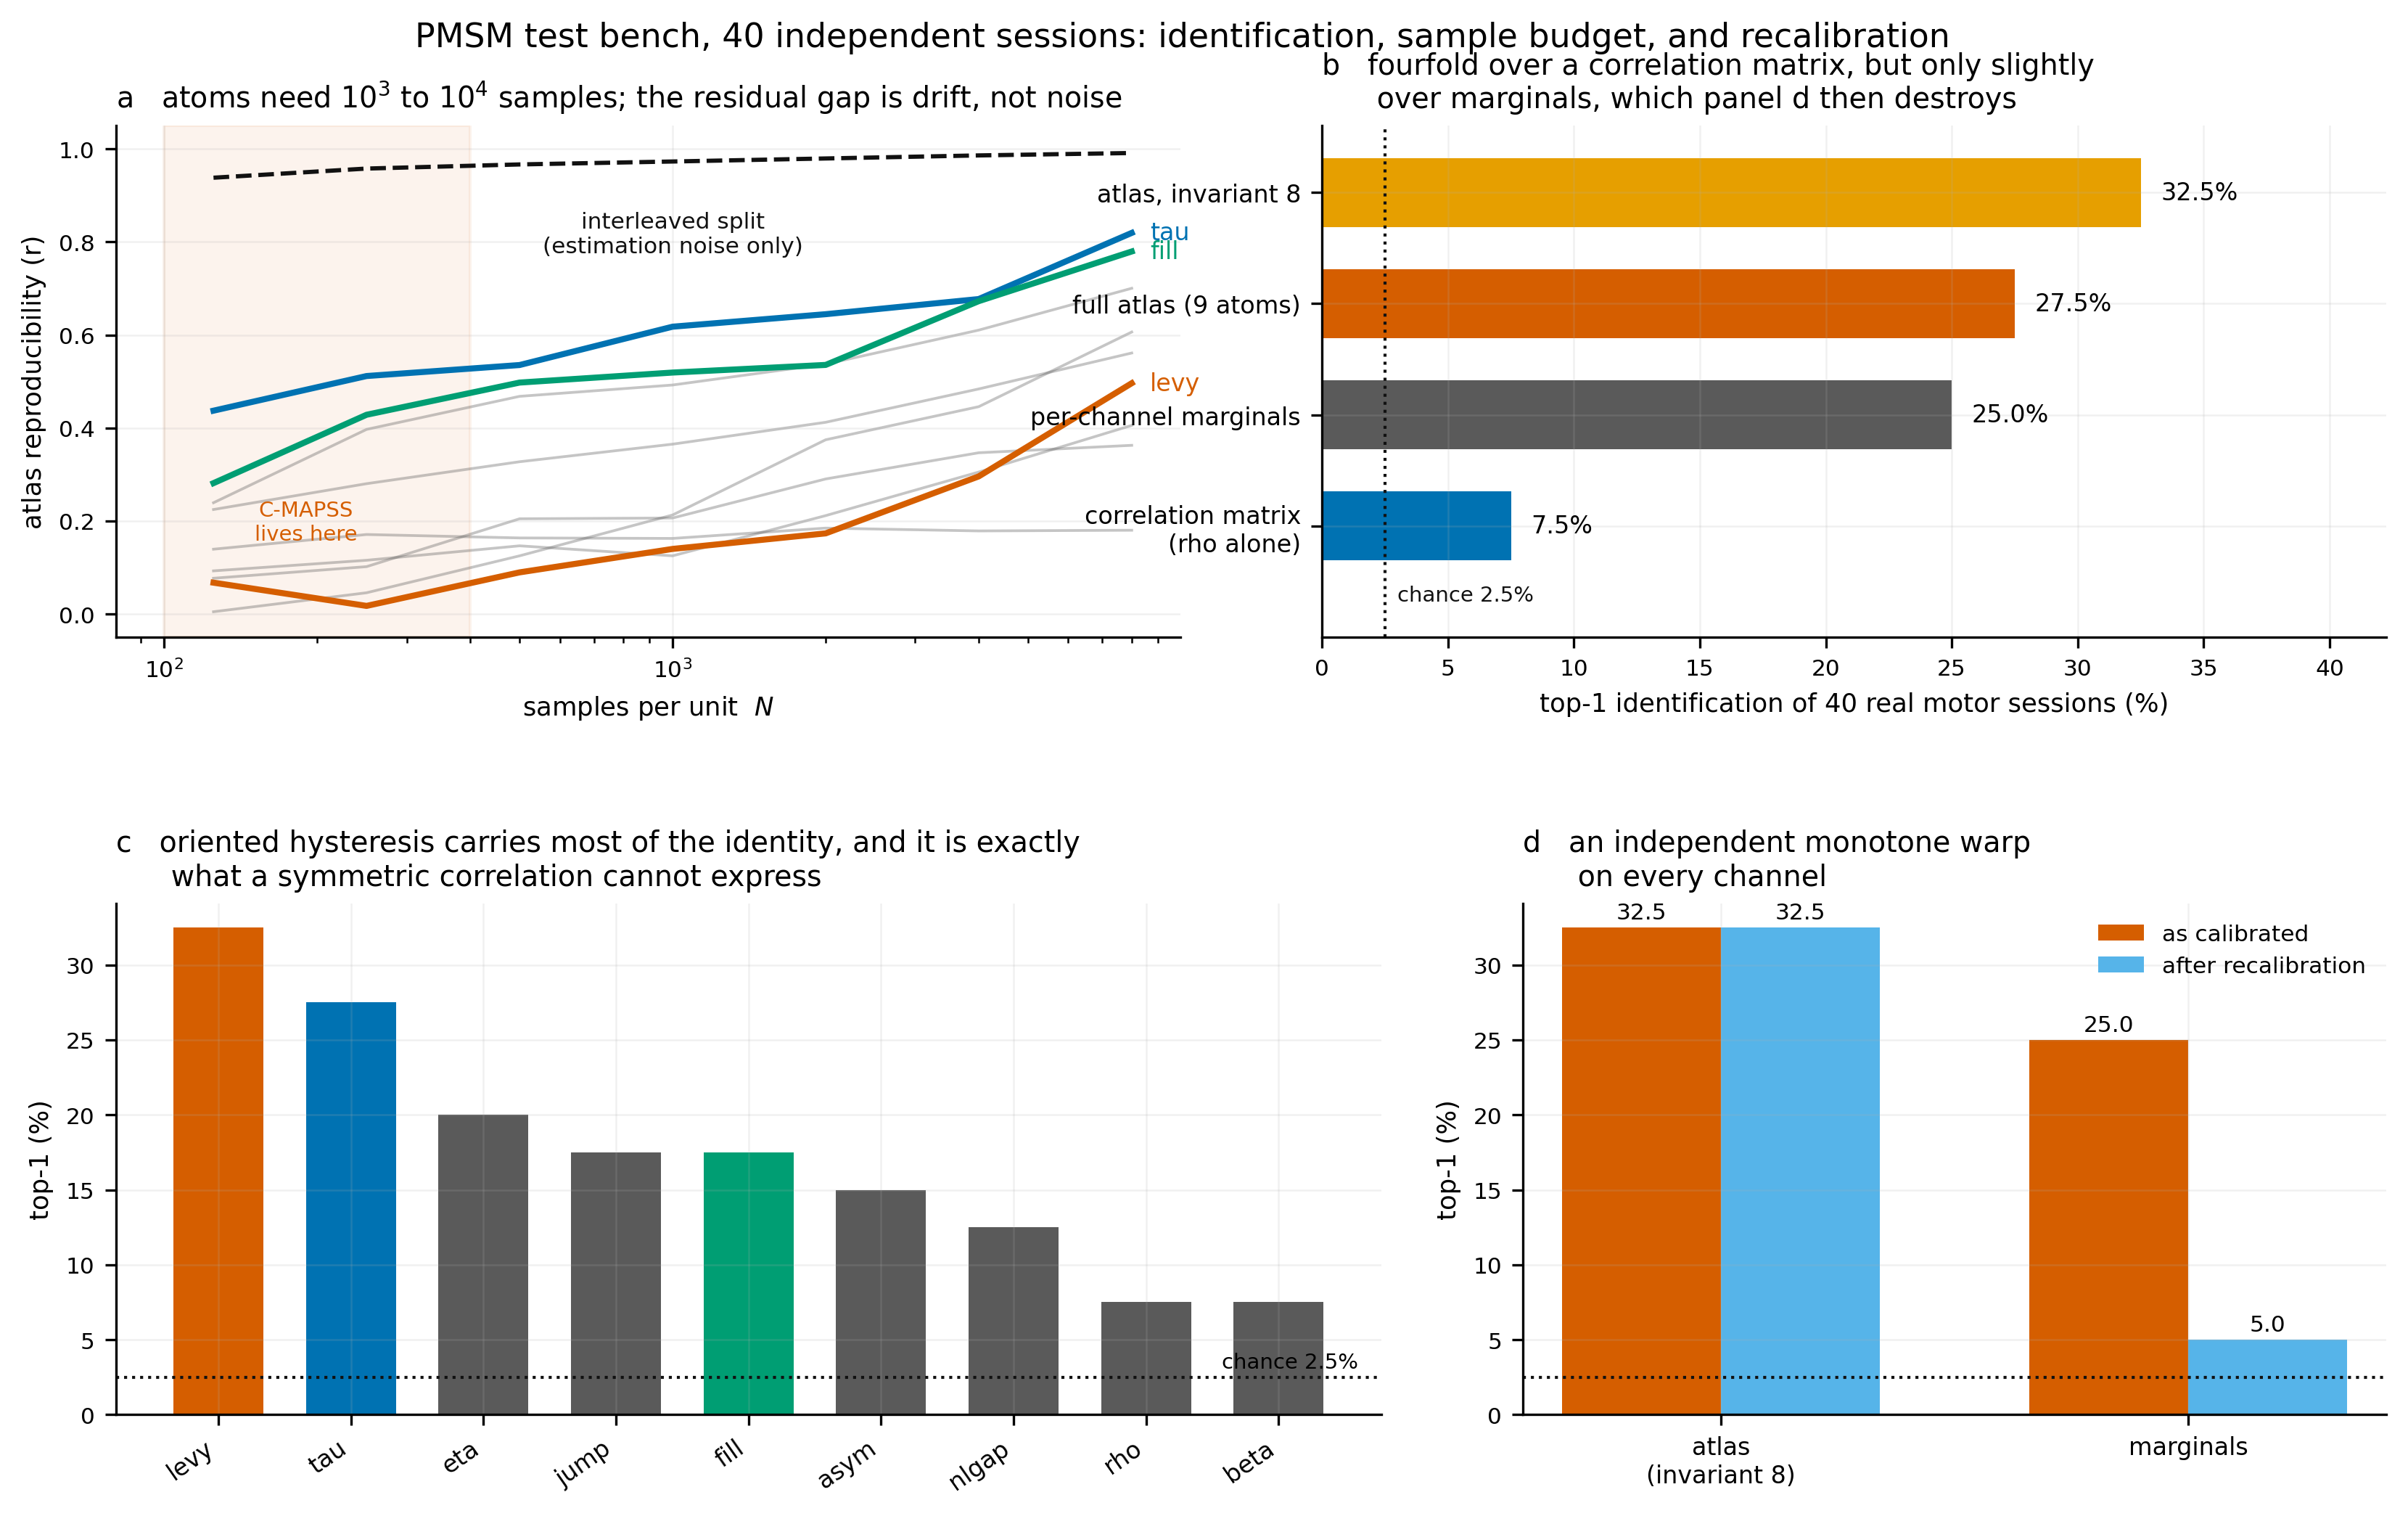
\includegraphics[width=\textwidth]{../atlas/fig2_results.png}
\caption{\textbf{a} Atlas reproducibility against samples per unit, with three
atoms highlighted and the rest in grey. The dashed line is an interleaved
split, which holds operating conditions fixed and so isolates estimation noise
alone; the gap below it is genuine non-stationarity. \textbf{b} Identification
by feature set. \textbf{c} Identification by single atom. \textbf{d} The same
after an independent strictly increasing warp on every channel.}
\end{figure}

\subsection{The telemetry budget}

Atoms are statistics and they need samples. Taking two disjoint windows from
one session and correlating the atlases estimated on each, agreement rises
monotonically with window length, from about $0.2$ at $N=125$ to $0.5$--$0.8$
at $N=4000$, still climbing. Splitting the same window into interleaved halves
instead, which holds the operating condition fixed and isolates estimation
noise alone, gives agreement of $1.00$ at $N=8000$. The gap between the two is
therefore not estimation error, it is genuine non-stationarity, which means
more data stops helping past roughly $10^4$ samples and what remains is the
machine actually changing.

This immediately explains a failure. On C-MAPSS, whose 709 units are around 200
cycles each, so each half-atlas is fitted from about 100 samples spread over
276 channel pairs, identification reaches 1.1\% against 0.14\% chance and the
full atlas scores below a plain correlation matrix at class assignment. That is
the noise regime, and the reproducibility curve locates it in advance without
reference to any downstream task, which makes it a cheap precondition a
practitioner can check before building anything.

\subsection{What invariance costs}

Conditioning the atlas on operating point can be done two ways. Absolute cells,
quantiles of raw torque with edges fitted once on the pooled fleet, presume
every machine is calibrated alike. Relative cells, quantiles of a rank space
load coordinate, are exactly invariant to recalibration. Absolute cells
identify better and relative cells survive re-instrumentation, and this is not
a tuning choice that can be optimised away, because a machine that simply runs
ten kelvin hotter than its siblings is identified by that fact, and an
invariant that is blind to absolute level is blind to it by construction.

\begin{table}[t]
\centering
\begin{tabular}{llrrrr}
\toprule
cells & basis & atlas top-1 & $\mathrm{levy}$ top-1 & after recalib. &
max atom shift \\
\midrule
1 & ---      & 27.5\% & 32.5\% & 32.5\% & $1.1\times10^{-1}$ \\
3 & absolute & 25.0\% & 35.0\% & 10.0\% & $9.1\times10^{0}$ \\
3 & rank     & \textbf{30.0\%} & 27.5\% & 25.0\% & $6.1\times10^{-1}$ \\
5 & absolute & 22.5\% & \textbf{42.5\%} & 10.0\% & $9.2\times10^{0}$ \\
5 & rank     & 22.5\% & 22.5\% & 22.5\% & $9.4\times10^{-1}$ \\
\bottomrule
\end{tabular}
\caption{Conditioning on operating point, with cells cut either on an absolute
load channel or on a rank space load coordinate. Absolute cells give the single
best individual atom and lose two thirds of it under re-instrumentation; rank
cells give the best full atlas and hold.}
\label{tab:cells}
\end{table}

Table~\ref{tab:cells} makes the trade concrete. Cutting cells on absolute load
produces the best single atom anywhere in this study, $\mathrm{levy}$ at
$42.5\%$, and loses three quarters of it the moment the channels are relabelled.
Cutting them in rank space gives the best full atlas at $30.0\%$ and barely
moves. Neither dominates, and which one is right depends on a fact about the
deployment rather than about the method.

We therefore report the atlas and a separate calibration block, per channel
median and interquartile range, rather than folding them together. Their union
is a strict superset of both and inherits the fragility of the weaker one, so
the choice belongs to the practitioner and depends on whether the fleet is
co-calibrated and stays that way.

The same tension has a sharp local form in the jump atom. Discontinuity is a
statement about magnitudes, and rank space discards magnitudes, so the jump
atom is the one place where the invariance requirement measurably costs
measurement power. It is the weakest of the nine, and we report it as such.

\subsection{The index of operators}

A unit's atlas is a vector over that unit's own channel pairs, so a 12 channel
motor bench and a 24 channel turbofan produce atlases of different length and
cannot be compared at all. That is a real obstacle to any class level claim,
and the fix is to stop treating the atlas as a vector over pairs and start
treating it as a distribution over pairs. Taking nine fixed quantiles of each
atom across all pairs gives 81 numbers whatever the channel count, and those 81
numbers say what kind of relational geometry a machine has rather than which
particular pair does what.

Across six classes, a permanent magnet motor bench, a metro air compressor, two
fault conditions of a water circulation pump rig, a turbofan, and windows of a
basket of traded assets, the profile assigns class at $93.6\pm1.4\%$ against a
$28.6\%$ majority, with every record strided to the same 400 samples. Holding
the budget at 900 samples instead, which the shorter records cannot meet and
which therefore leaves four classes, gives $97.2\pm2.3\%$.

Equalising the record length is not a detail, it is the experiment. Two of the
nine atoms are sensitive to how the data was acquired rather than to what the
machine did, since $\mathrm{fill}$ counts occupied grid cells and therefore
grows with record length, and $\tau$ is an autocorrelation time measured in
samples and therefore tracks the logging rate. A classifier handed unequalised
records can separate a motor bench from a compressor by how fast each was
logged, and will score well doing it while learning nothing. Dropping both
atoms entirely leaves accuracy at $94.3\pm2.9\%$, so the class signal is not an
acquisition artefact.

The confusion matrix locates the difficulty where it should be. The motor
bench, the compressor and the traded assets are never confused with anything.
Every error falls between the two fault conditions of the same pump rig, which
is the one pair of classes sharing hardware, instrumentation and logging rate,
differing only in what is wrong with the valve.

We include the traded assets deliberately and claim nothing more from them than
this. A market is not a machine and has no thermal network, but the atom
vocabulary is defined on any set of jointly sampled channels, and the fact that
market windows form a clean class under the same 81 numbers says the
construction is not quietly encoding something specific to rotating machinery.

\begin{figure}[t]
\centering
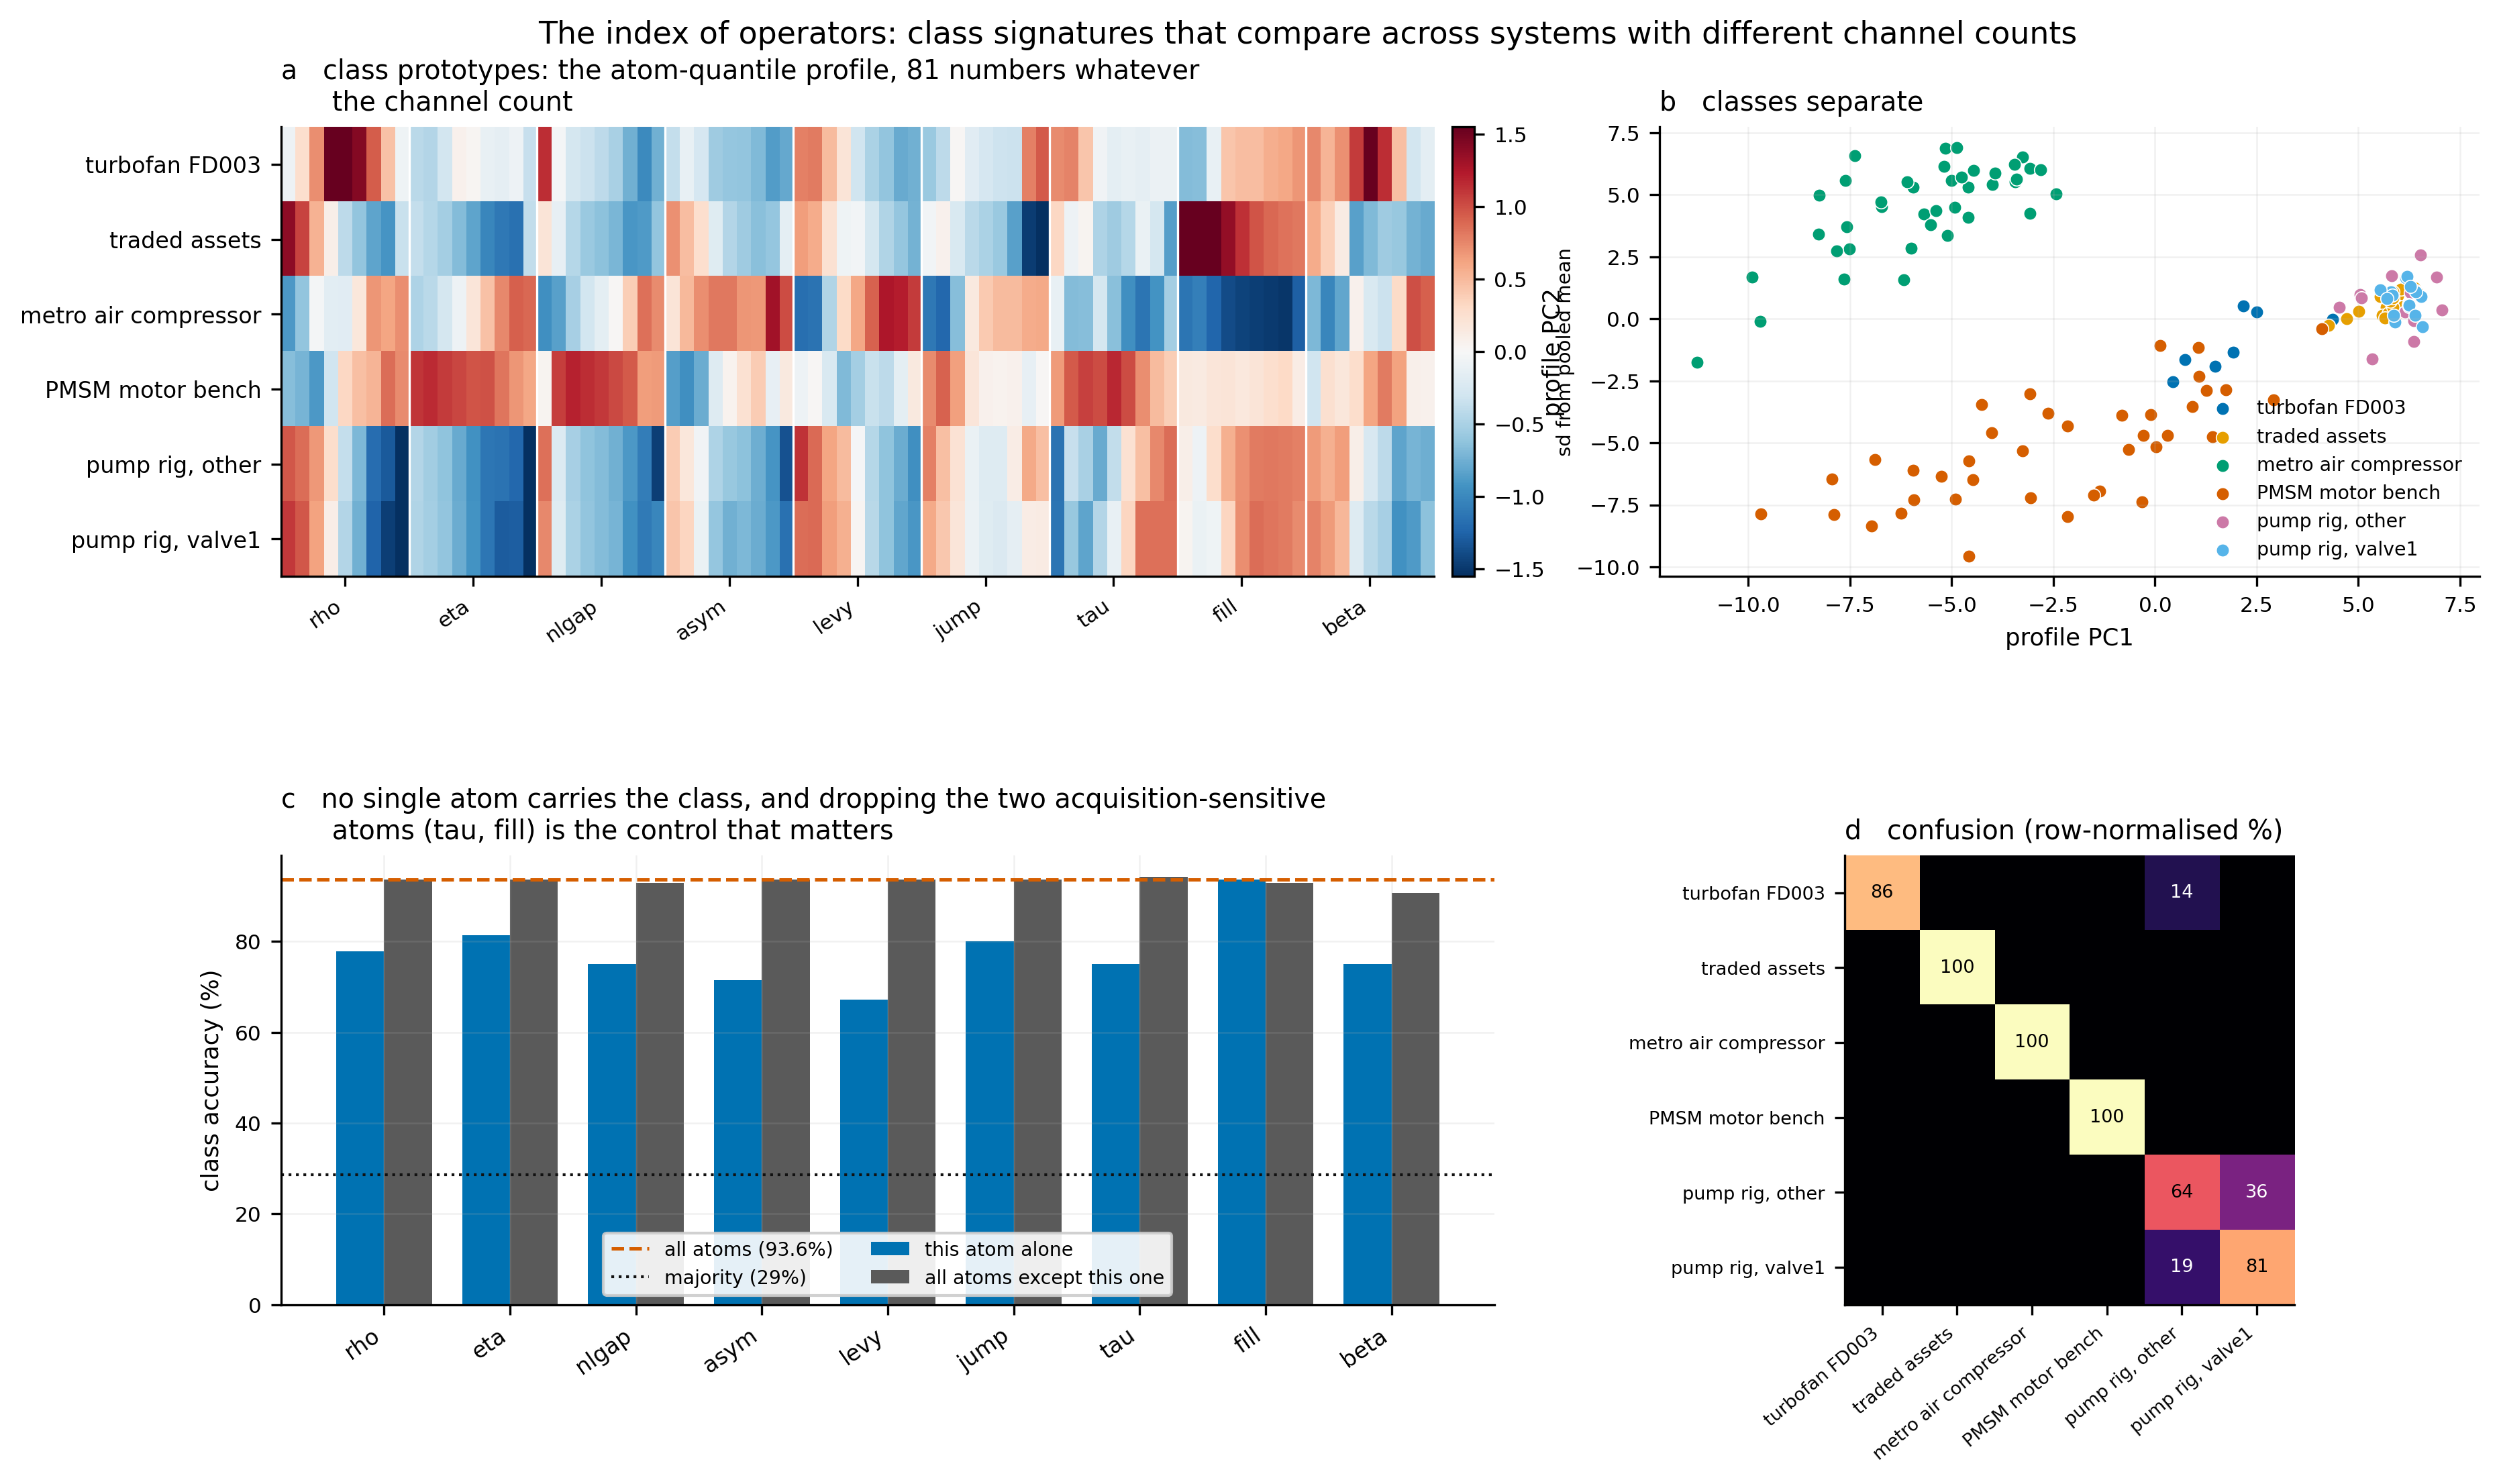
\includegraphics[width=\textwidth]{../atlas/fig3_classes.png}
\caption{\textbf{a} Class prototypes as atom-quantile profiles, 81 numbers
whatever the channel count. \textbf{b} The same profiles in two principal
components. \textbf{c} Leave-one-atom-out and one-atom-only accuracy; the
control that matters is dropping $\tau$ and $\mathrm{fill}$ together, the two
atoms sensitive to how the data was acquired rather than to what the machine
did. \textbf{d} Confusion. Every error falls between two fault conditions of
the same pump rig.}
\end{figure}

\subsection{Six real industrial systems}\label{sec:real}

\begin{figure}[t]
\centering
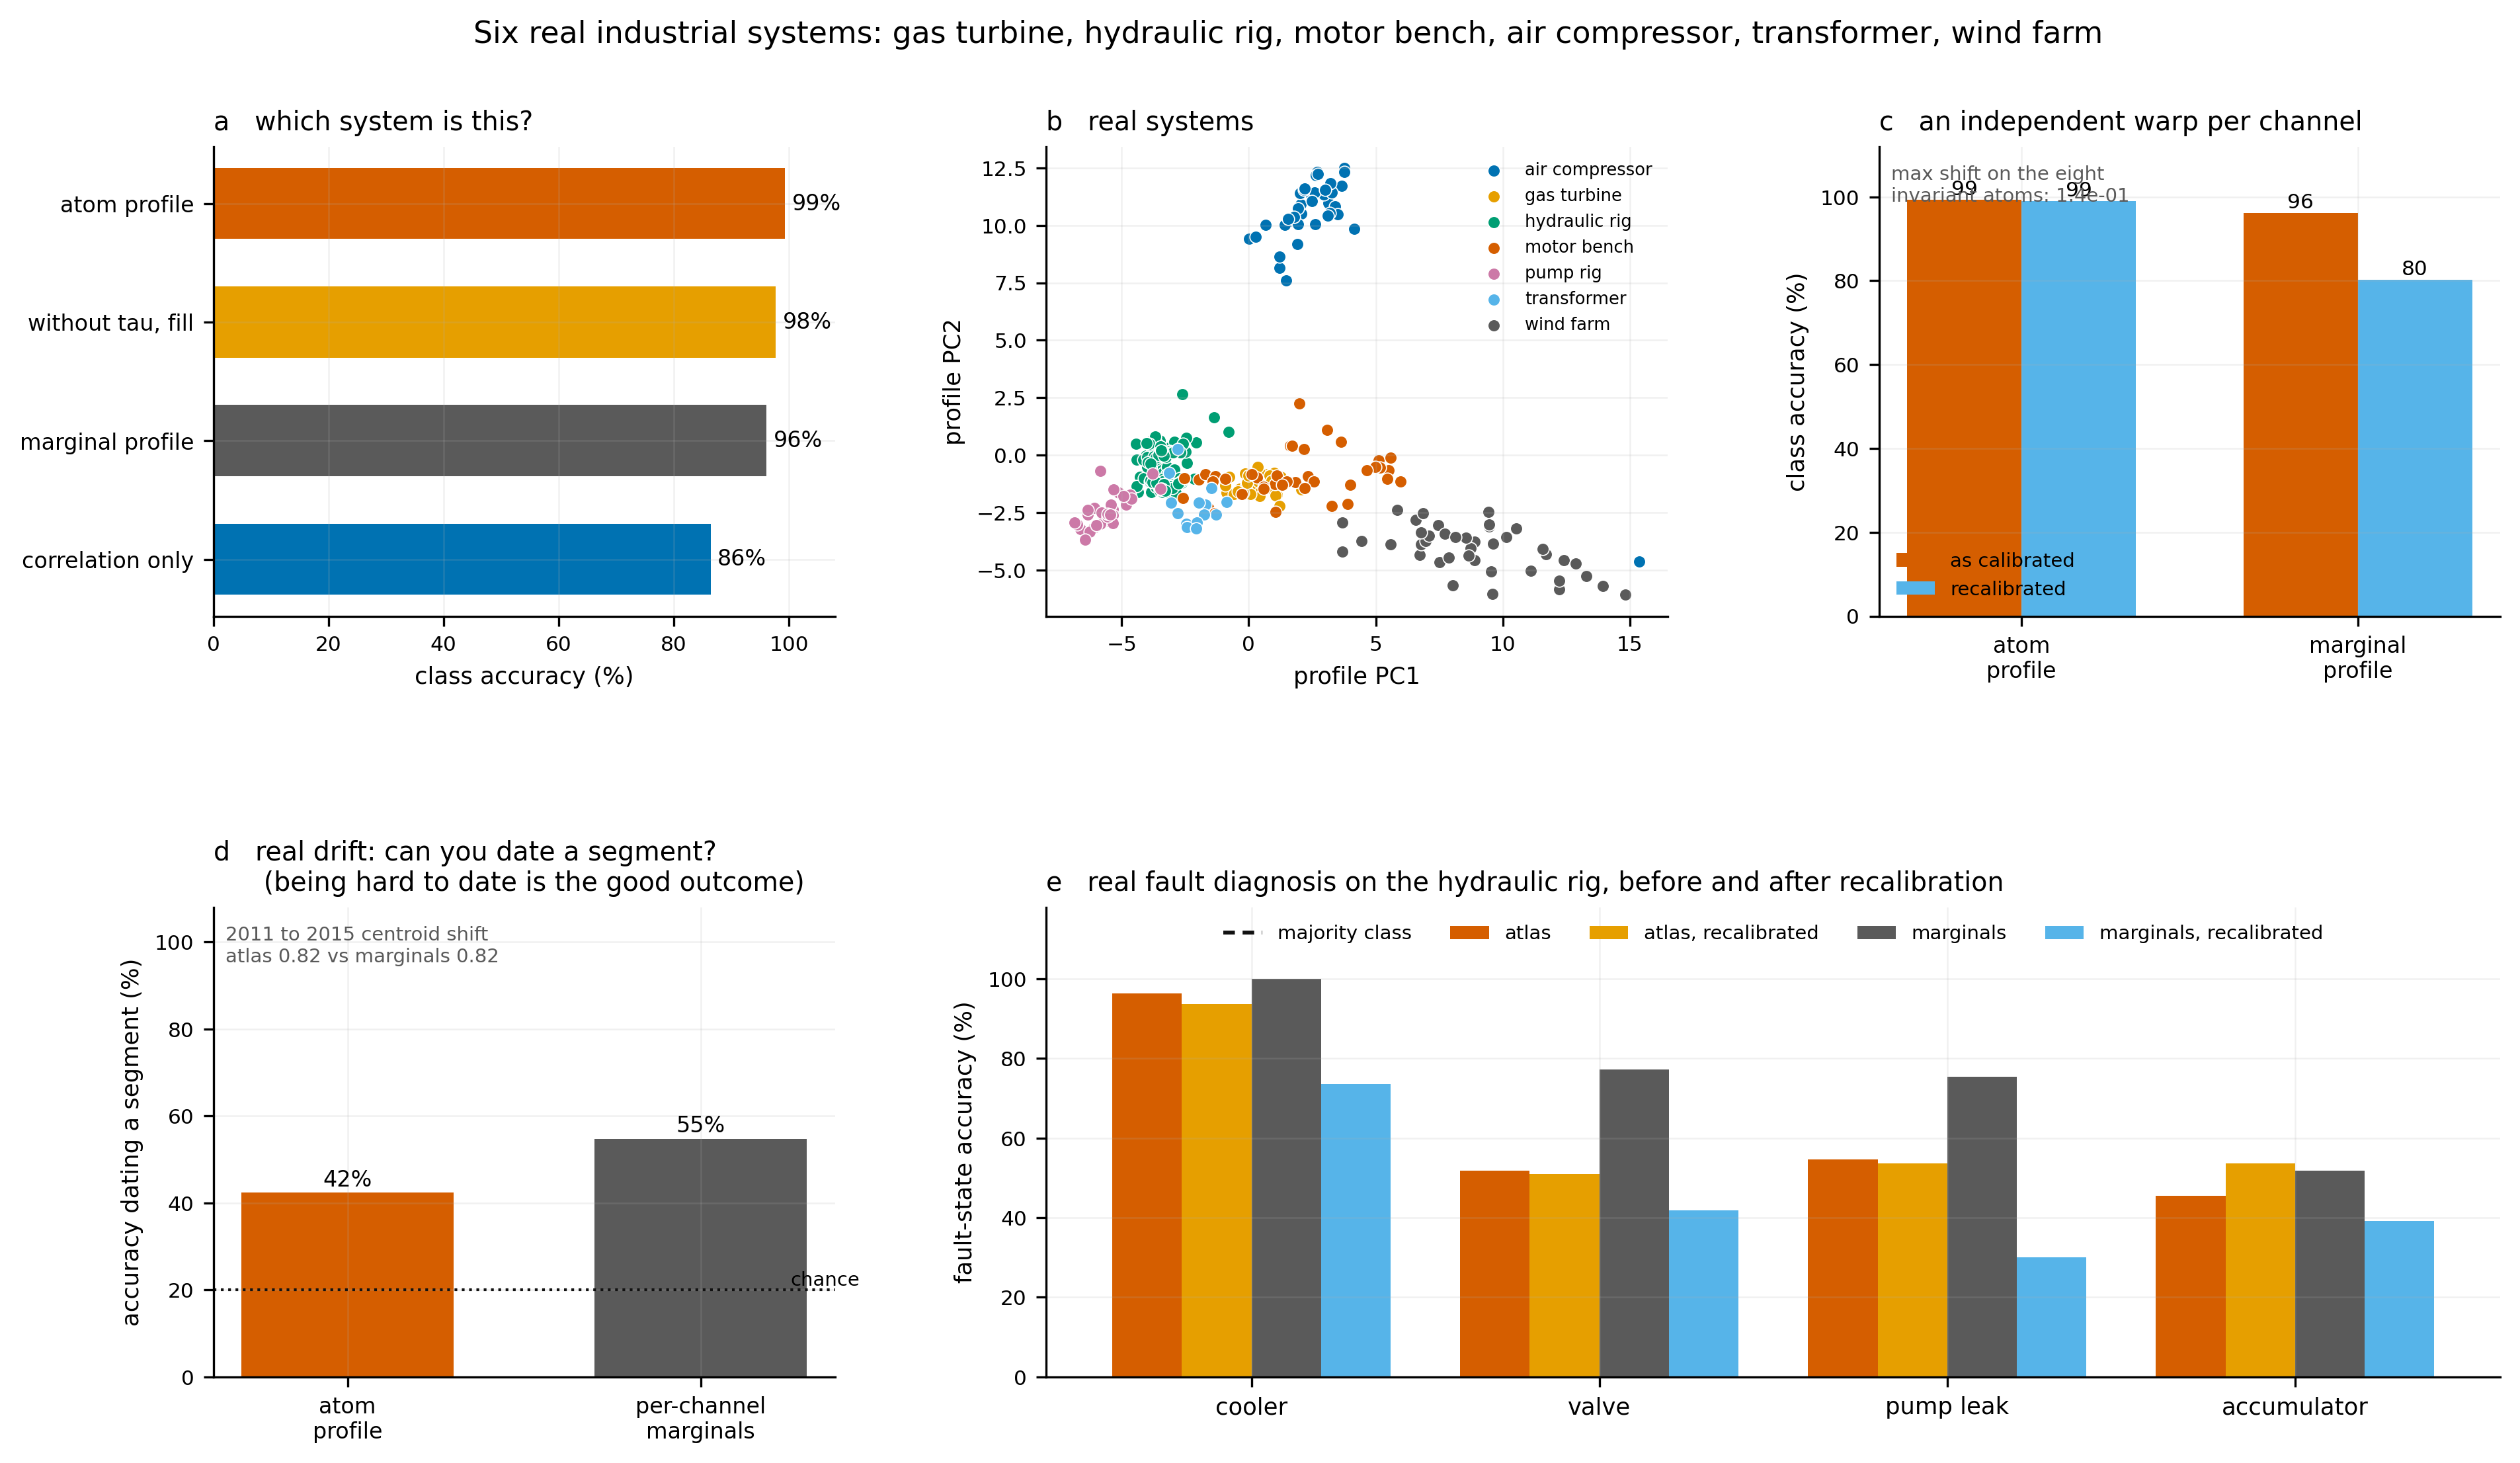
\includegraphics[width=\textwidth]{../atlas/fig4_real.png}
\caption{Real hardware only. \textbf{a,b} Class separation and the profile
embedding. \textbf{c} An independent strictly increasing warp per channel.
\textbf{d} Real five-year drift on one gas turbine. \textbf{e} Fault diagnosis
on the hydraulic rig against the majority-class floor, which two of the four
components do not clear.}
\end{figure}

Everything above rests on one motor bench and on simulation. Here the same
construction meets six real industrial systems at once: an industrial gas
turbine logged hourly for five years, a hydraulic test rig with 17 sensors and
documented fault conditions, a permanent magnet motor bench, a metro air
compressor, an electricity transformer, and a wind farm SCADA feed. Channel
counts run from 4 to 17, so the comparison uses the atom-quantile profile, and
the marginal baseline is made commensurable the same way, by taking quantiles
across channels rather than concatenating them.

\emph{Class separation.} The profile assigns which of the six systems a record
came from at $98.9\pm0.9\%$ against a $39.4\%$ majority, where the marginal
profile reaches $96.1\pm2.1\%$ and a correlation profile alone $85.7\pm4.4\%$.
Dropping the two acquisition-sensitive atoms leaves $97.9\pm0.7\%$.

\emph{Recalibration.} Under an independent strictly increasing warp on every
channel of every system, the atlas is unchanged at $98.9\%$ while the marginal
profile falls to $83.9\%$. The largest movement of any invariant atom is
$1.4\times10^{-1}$ rather than the exact zero seen on double precision data,
and the cause is the one already documented in the methods: three of the six
systems are stored in single precision, so a warp segment with slope below one
merges adjacent quantisation levels and the realised map is no longer injective.
The classification is unaffected, but the invariance is exact only where the
stored data has room for it to be.

\emph{Real drift, and a prediction of ours that failed.} The gas turbine gives
five years of genuine asset ageing, sensor ageing and maintenance on one
machine. We expected the atlas to move less than per channel statistics under
that drift. It does not. The centroid shift from 2011 to 2015 is $0.819$ for the
atlas against $0.817$ for the marginals, which is the same number. What does
differ is datability: a classifier recovers the year of a held out segment at
$54.8\pm8.0\%$ from marginals against $42.4\pm10.5\%$ from the atlas, on 33
segments, which is too few to lean on.

The right reading is that recalibration and ageing are different things and we
had conflated them. A recalibration relabels the same physics, and the atlas is
exactly invariant to it by construction. Ageing changes the physics: compressor
fouling genuinely alters the relationship between inlet temperature and
discharge pressure, and an honest relational description should move when that
happens. The atlas is invariant to the instrument and sensitive to the machine,
which is the desirable pairing, but it is not the claim that relational
descriptors resist drift, and that claim should not be made.

\emph{Fault diagnosis, where the atlas mostly loses.} The hydraulic rig ships
ground-truth condition labels for four components. Results are in
Table~\ref{tab:fault} and they are not flattering.

\begin{table}[t]
\centering
\begin{tabular}{lrrrrr}
\toprule
component & majority & atlas & marginals & atlas, recal. & marginals, recal. \\
\midrule
cooler       & 33.6\% & 96.4\% & \textbf{100.0\%} & 93.6\% & 73.6\% \\
valve        & 50.9\% & 51.8\% & \textbf{77.3\%}  & 50.9\% & 41.8\% \\
pump leak    & 55.5\% & 54.5\% & \textbf{75.5\%}  & 53.6\% & 30.0\% \\
accumulator  & 36.4\% & 45.5\% & \textbf{51.8\%}  & 53.6\% & 39.1\% \\
stable flag  & ---    & 85.5\% & 84.5\%           & 86.4\% & 55.5\% \\
\bottomrule
\end{tabular}
\caption{Hydraulic rig, $n=110$ records. Per channel statistics win on every
component before recalibration, and the atlas fails to clear the majority class
on two of them.}
\label{tab:fault}
\end{table}

Per channel statistics beat the atlas on all four components, and on valve
condition and pump leakage the atlas does not clear the majority class at all,
at $51.8\%$ against $50.9\%$ and $54.5\%$ against $55.5\%$. Reporting those two
as robustness successes because they barely move under recalibration would be
meaningless, since there is nothing there to preserve.

The pattern across components is physically coherent and is the useful output
of this experiment. Cooler condition is a change in a \emph{coupling}, since a
degraded cooler changes how power draw maps to temperature rise, and the atlas
gets $96.4\%$ on it. Valve switching and pump leakage are changes in
\emph{level}, since they shift absolute pressures and flows, and a description
that discards magnitude cannot see them. The design rule that follows is
specific enough to act on: use relational atoms for faults that alter couplings,
and keep per channel statistics for faults that alter levels. The two are
complementary, and the recalibration column is the reason to carry both rather
than only the second.

\subsection{A fleet with known physics}\label{sec:fleet}

Public fleet datasets cannot answer the question that matters, because nobody
knows the true bearing friction of unit 47. We therefore simulate fleets of 80
individual machines on each of three MuJoCo Menagerie arms, a UR5e, a Franka
Panda and a KUKA iiwa14, each carrying an injected two node joint thermal
network with derating and a hysteretic drive trip. Each unit is given a fixed
physical identity, its payload, winding to housing and housing to ambient
thermal resistances, winding resistance, bearing friction, servo gain, and how
unevenly those load onto its joints. Each unit is then run for several episodes
whose workload, duty cycle, ambient temperature and excitation, is drawn fresh
every time. Atlases are built from a unit's early episodes and matched against
its later ones, so any similarity is a property of the machine and not of the
task.

Three results follow, and only the third is unambiguous.

\begin{table}[t]
\centering
\begin{tabular}{lrrrrrr}
\toprule
& \multicolumn{2}{c}{identification} & \multicolumn{2}{c}{after recalibration}
& \multicolumn{2}{c}{workload decode ($R^2$)} \\
\cmidrule(lr){2-3}\cmidrule(lr){4-5}\cmidrule(lr){6-7}
platform & atlas & marginals & atlas & marginals & atlas & marginals \\
\midrule
UR5e    & 11.2\% & 10.0\% & \textbf{11.2\%} & 3.8\% & $0.04$ / $-0.05$ & $0.82$ / $0.99$ \\
Panda   & 15.0\% & 17.5\% & \textbf{15.0\%} & 6.2\% & $0.52$ / $-0.07$ & $0.89$ / $0.95$ \\
iiwa14  &  6.2\% &  2.5\% & \textbf{6.2\%}  & 1.2\% & $0.14$ / $-0.11$ & $0.84$ / $0.72$ \\
\bottomrule
\end{tabular}
\caption{Simulated fleets of 80 units each, chance $1.2\%$. Workload decode is
duty cycle and ambient temperature, neither of which is a property of the
machine. Recalibration leaves the atlas numerically unchanged, to
$0.0\times10^{0}$ on all eight invariant atoms on all three platforms.}
\label{tab:fleet}
\end{table}

Identification is a wash. The atlas beats per channel marginals on two
platforms and loses on the third, at 11.2 against 10.0, 15.0 against 17.5, and
6.2 against 2.5 percent. On a fleet whose units differ mostly in payload, which
is an absolute level property, there is no reason it should have won, and it
did not.

Recovering the true physics is likewise split, and in the direction the
invariance argument predicts. Payload is decoded at $R^2=0.61$ from the atlas
against $0.99$ from a per channel calibration block, because hanging five
kilograms on a flange moves torque magnitudes and the invariant atlas has
discarded magnitudes by construction. Bearing friction goes the other way on
the iiwa14, $0.36$ from the atlas against a divergent $-5.49$ from marginals.

The workload control is where the two representations separate completely, and
it is the result we would keep if we could keep only one. Duty cycle and
ambient temperature are properties of the task, not of the machine, and a
representation that encodes them is to that extent a duty detector wearing the
costume of a machine fingerprint. Per channel marginals decode ambient
temperature at $R^2$ of $0.99$, $0.95$ and $0.72$, and duty at $0.82$, $0.89$
and $0.84$. The atlas decodes ambient temperature at $-0.05$, $-0.07$ and
$-0.11$, which is to say no better than predicting the mean, and duty at
$0.04$, $0.52$ and $0.14$. Whatever the atlas is carrying, it is not the
workload, and whatever the marginal baseline is carrying, a large part of it
is.

That reframes the identification wash rather than excusing it. The two
representations reach similar identification scores while encoding almost
disjoint information, and only one of them is still standing after the
instrumentation changes.

Finally, within class atlas variation is genuinely low dimensional. Across the
three fleets, 80\% of the variance sits in 43 to 45 directions out of 12{,}555
to 17{,}010, which is the quantitative form of the claim that a class prototype
is fine tuned to a unit by moving a small number of knobs. Class assignment
across the three arms is $100\%$.

\subsection{Does the identity help prediction?}

Identification shows the atlas carries unit identity. It does not show the
identity is useful, and on the test we ran it is not.

We pretrain a short horizon forward model on a fleet, predicting joint velocity
and winding temperature ten steps ahead from the current state and a causal
EWMA history, hold out units never seen in pretraining, and adapt to each with
$N$ samples of its own. Conditioning the model on the unit's atlas code is
compared against no conditioning, against the calibration block, against the
unit's \emph{true} physical parameters, and against training from scratch.

Pretraining works and matters, since scratch training reaches a test error of
$0.845$ at $N=200$ against $0.129$ for the pretrained pooled model. Unit
conditioning does not. At $N=200$ the pooled model with no unit information at
all is best at $0.129$, the calibration block gives $0.149$, the atlas gives
$0.168$, and the oracle, which is handed the true payload and thermal
resistances and bearing friction, gives $0.160$.

The oracle is the informative arm. If conditioning on true physical parameters
does not beat conditioning on nothing, then the failure is not that the atlas
recovers the identity badly. It is that the identity is redundant for this
task, because a forward model that already sees the current state and a causal
history of it is implicitly told what kind of machine it is on, and being told
again in a separate input costs a few dimensions and buys nothing. We report
this as a negative result about short horizon forward prediction specifically,
not about every possible use of a unit code, but it is the use most often
assumed and it did not survive contact.

\section{Methods}

\subsection{Atom computation}

All eight rank atoms are computed from the channelwise rank transform with ties
averaged, mapped to $(0,1)$. The whole atlas is $O(d^2 n)$ and consists of
matrix products, bincounts and rank transforms, with no pairwise distance
statistic anywhere, which is what keeps it affordable at $d=40$ and
$n=10^5$. Three implementation choices are load bearing.

The correlation ratio $\eta$ and the exponent $\beta$ both need per-bin
aggregates of every channel at once. These are computed as one-hot matrix
products rather than with scatter-add, which in NumPy falls back to an
unbuffered element loop and dominated the entire atlas before it was replaced.

The L\'evy denominator needs an absolute value inside the sum and therefore
cannot be a single matrix product. It is accumulated over time blocks sized by
a fixed memory budget rather than a fixed row count, so the temporary stays
around 16\,MB whether $d$ is 8 or 40 instead of scaling with $d^2$.

The occupancy atom counts occupied cells with a bincount rather than by calling
unique, which is $O(n)$ instead of $O(n\log n)$ and mattered at large $n$.

\subsection{Cells}

Conditional atlases partition a record by operating point. The load coordinate
is the mean of the per channel ranks of a designated channel group, torque for
the motor and the joint torques for the arms, and cells are quantiles of it.
Both choices are forced. A raw summed load is not invariant, because an
independent monotone warp per channel does not commute with a sum, so warped
samples cross the cell boundaries and the conditional atlas moves even though
every atom in it is invariant. Averaging per channel ranks fixes this exactly.
Fitting the direction per unit, as an earlier version did with a leading
principal component, is worse still, because a principal direction is defined
only up to sign, so half a fleet has its cells in reverse order and ``cell 1''
is not a shared operating condition at all.

\subsection{Recalibration model}

A simulated re-instrumentation applies an independent strictly increasing map
to each channel, drawn as a monotone piecewise linear function through seven
random increasing knots with every segment slope bounded below at $0.3$,
composed with a random positive gain and offset. The slope floor is the point.
A composition of a power law and a logistic squash is monotone on paper, but
with the exponent drawn as $\exp(\mathcal{N}(0,0.8))$ it routinely reaches
$10$, which sends most of the unit interval below $10^{-10}$ and onto the flat
tail of the logistic, collapsing thousands of distinct readings onto a single
float. That is information destruction rather than relabelling, and no
invariant of any kind survives it.

One caveat is worth stating precisely. The invariance is exact for injective
maps. Real telemetry is stored in single precision, so a warp with a segment
slope below one can merge adjacent quantisation levels, and where it does the
map realised on the stored data is not injective and the atoms move by a
bounded amount. On continuous double precision data the measured shift of all
eight invariant atoms is $0.00\times10^{0}$ exactly. On the single precision
motor bench, under warps aggressive enough to merge roughly $10\%$ of the
distinct torque levels, the largest shift across all eight is $0.11$, and the
identification result is unchanged at $32.5\%$.

\subsection{Identification protocol}

Atlases are built from the first half of a record and matched against atlases
from the second half. Features are $z$-scored on the pooled set, $\ell_2$
normalised per unit, and matched by cosine similarity. Top-1 is the fraction of
units whose own second half is their nearest neighbour among all candidates,
and percentile rank is the mean position of the true match in the ranked
candidate list, so chance is $1/n$ and $50\%$ respectively.

\subsection{Class profiles}

Each record contributes the nine quantiles $\{0.02,0.10,0.25,0.40,0.50,0.60,
0.75,0.90,0.98\}$ of each atom across all its pairs. Every record is strided to
a common length before profiling, for the reason given in the results.
Classification is multinomial logistic regression on standardised profiles with
stratified five fold cross validation.

\section{Discussion}

The useful way to read these results is as a statement about where relational
geometry is worth its cost. On a fleet that is stable and co-calibrated, per
channel statistics already carry most of what identifies a machine, and a
practitioner who adds an atlas will get a modest improvement for a real
increase in complexity. The moment instrumentation changes, and it does change,
because sensors are replaced and drives are re-tuned and thermocouples are
re-zeroed, everything built on magnitudes is invalidated at once while the
atlas is untouched. That is a narrow claim and it is the one we can support.

The second reading concerns what kind of quantity carries machine identity. It
is not correlation. A correlation matrix is the reduced form of our own
construction and it recovers a quarter of the identification the full atom set
does, and the gap is dominated by a single antisymmetric quantity. Symmetric
descriptors of a pair, which is what almost the entire relational feature
literature uses, cannot express which of two coupled channels leads. In a
system whose defining behaviour is a lag with a direction, that is the
information worth having, and it is free once the pair is being looked at
anyway.

Three limitations deserve to be stated plainly rather than left for a reader to
find. The jump atom is weak, and it is weak for a principled reason: a
discontinuity is a claim about magnitudes and rank space discards magnitudes,
so the requirement that made the other atoms invariant is exactly what costs
this one its power. The sample budget is real and cheap to check, which makes
it a genuine precondition rather than a caveat, but it does rule the method out
for short-record fleets. And the class signature, being a distribution over
pairs, deliberately throws away which pair does what, so it says what kind of
machine this is and not which part of it is misbehaving.

The third reading is a negative one and it deserves as much weight as the
others. A unit code that demonstrably carries unit identity did not improve
short horizon forward prediction for that unit, and neither did the true
physical parameters. That is not a failure of the atlas, it is a fact about the
task: a model that already sees a causal history of the state has been told
what machine it is on, and telling it again is redundant. The practical
consequence is that anyone proposing to condition a predictor on a learned
machine embedding should run the oracle arm first, because if ground truth
parameters do not help, no embedding of them will.

What that leaves is a representation whose value is in identification,
auditing and transfer rather than in accuracy. Knowing which machine a record
came from, knowing that the answer does not change when the sensors are
replaced, and knowing that the answer is not secretly the duty cycle, are worth
having on their own. The workload control is the cleanest evidence for that
last point, and it is the experiment we would most encourage others to copy,
because a fingerprint that quietly encodes the task will pass every
identification benchmark and fail in the field.

\section{Data and code availability}

C-MAPSS and the PMSM bench are public Kaggle datasets. Robot models come from
MuJoCo Menagerie. All atlas code is released.

\end{document}
